\documentclass{standalone}
\usepackage{tikz}
\usetikzlibrary{patterns, positioning}
\usepackage[sfdefault]{ClearSans} %% option 'sfdefault' activates Clear Sans as the default text font
\usepackage[T1]{fontenc}

\begin{document}
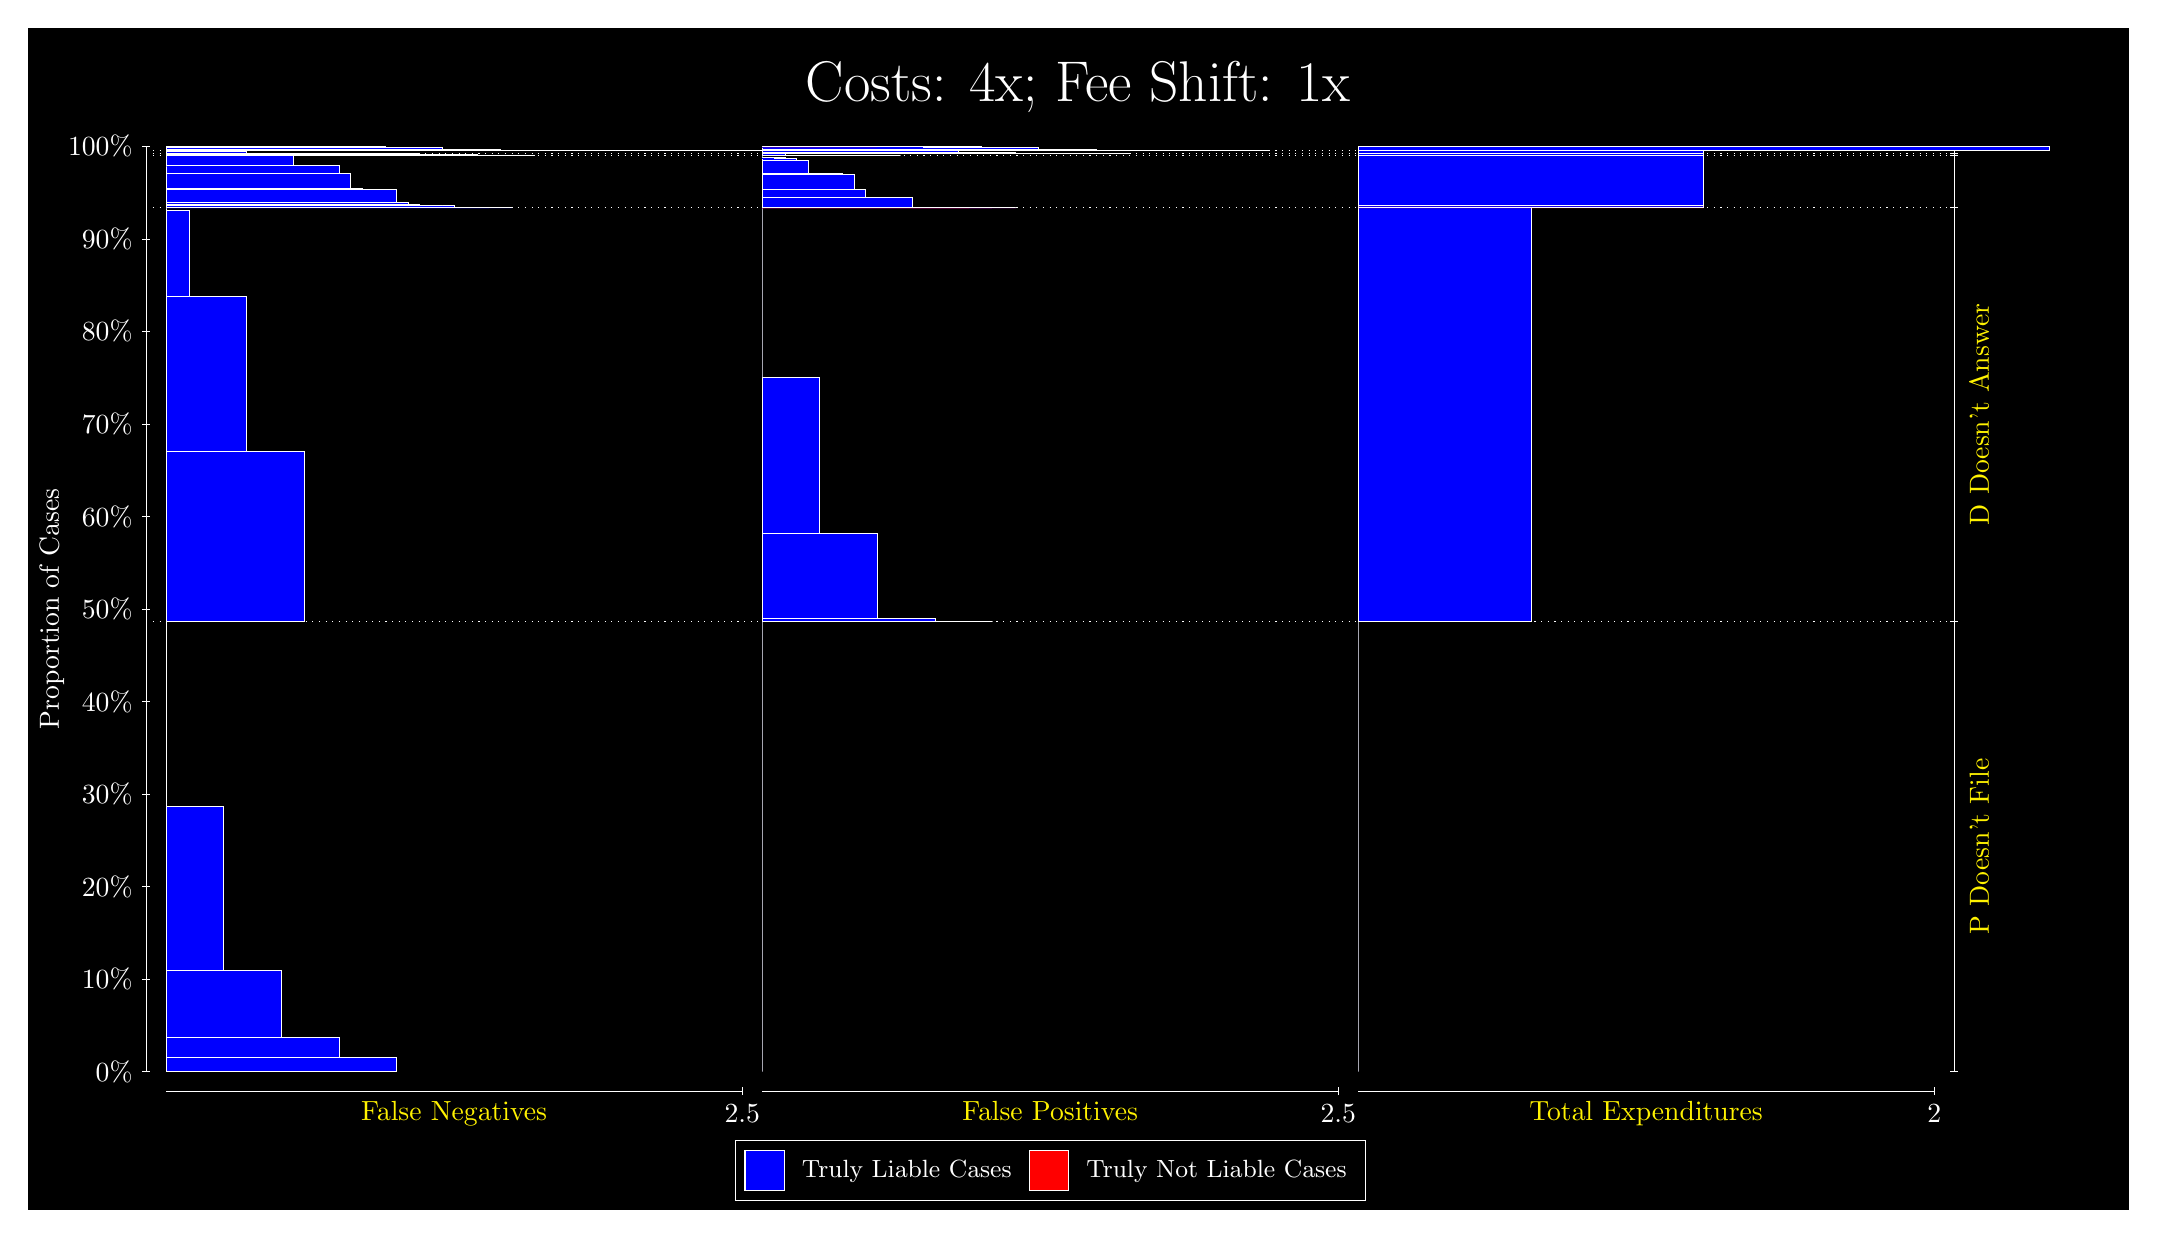
\begin{tikzpicture}
\draw[fill=black] (0,0) rectangle (26.667,15);
\draw[text=white] (0,13.5) rectangle (26.667,15) node[midway] {\huge Costs: 4x; Fee Shift: 1x};
\draw[white, very thin] (1.5,1.75) -- (1.5,13.5);
\node[rotate=90, text=white, anchor=center] at (0.3, 7.625) {Proportion of Cases};
\draw[white, very thin] (1.45,1.75) -- (1.55,1.75);
\node[text=white, anchor=east] at (1.45, 1.75) {0\%};
\draw[white, very thin] (1.45,2.925) -- (1.55,2.925);
\node[text=white, anchor=east] at (1.45, 2.925) {10\%};
\draw[white, very thin] (1.45,4.1) -- (1.55,4.1);
\node[text=white, anchor=east] at (1.45, 4.1) {20\%};
\draw[white, very thin] (1.45,5.275) -- (1.55,5.275);
\node[text=white, anchor=east] at (1.45, 5.275) {30\%};
\draw[white, very thin] (1.45,6.45) -- (1.55,6.45);
\node[text=white, anchor=east] at (1.45, 6.45) {40\%};
\draw[white, very thin] (1.45,7.625) -- (1.55,7.625);
\node[text=white, anchor=east] at (1.45, 7.625) {50\%};
\draw[white, very thin] (1.45,8.8) -- (1.55,8.8);
\node[text=white, anchor=east] at (1.45, 8.8) {60\%};
\draw[white, very thin] (1.45,9.975) -- (1.55,9.975);
\node[text=white, anchor=east] at (1.45, 9.975) {70\%};
\draw[white, very thin] (1.45,11.15) -- (1.55,11.15);
\node[text=white, anchor=east] at (1.45, 11.15) {80\%};
\draw[white, very thin] (1.45,12.325) -- (1.55,12.325);
\node[text=white, anchor=east] at (1.45, 12.325) {90\%};
\draw[white, very thin] (1.45,13.5) -- (1.55,13.5);
\node[text=white, anchor=east] at (1.45, 13.5) {100\%};

\draw[white, very thin] (24.457,1.75) -- (24.457,13.5);
\draw[white, very thin] (24.407,1.75) -- (24.507,1.75);
\node[anchor=west] at (24.407, 1.75) {};
\draw[white, very thin] (24.407,7.4668) -- (24.507,7.4668);
\node[anchor=west] at (24.407, 7.4668) {};
\draw[white, very thin] (24.407,12.723) -- (24.507,12.723);
\node[anchor=west] at (24.407, 12.723) {};
\draw[white, very thin] (24.407,13.386) -- (24.507,13.386);
\node[anchor=west] at (24.407, 13.386) {};
\draw[white, very thin] (24.407,13.414) -- (24.507,13.414);
\node[anchor=west] at (24.407, 13.414) {};
\draw[white, very thin] (24.407,13.45) -- (24.507,13.45);
\node[anchor=west] at (24.407, 13.45) {};
\draw[white, very thin] (24.407,13.5) -- (24.507,13.5);
\node[anchor=west] at (24.407, 13.5) {};

\draw[white, very thin, fill=blue] (1.75,1.75) rectangle (4.6775,1.9315);
\draw[white, very thin, fill=blue] (1.75,1.9315) rectangle (3.9457,2.1901);
\draw[white, very thin, fill=blue] (1.75,2.1901) rectangle (3.2138,3.0393);
\draw[white, very thin, fill=blue] (1.75,3.0393) rectangle (2.4819,5.1195);
\draw[white, very thin, fill=red] (1.75,5.1195) rectangle (1.75,5.1195);
\draw[white, very thin, fill=blue] (1.75,5.1195) rectangle (1.75,7.4668);
\draw[white, very thin, fill=blue] (1.75,7.4668) rectangle (3.5065,9.6264);
\draw[white, very thin, fill=blue] (1.75,9.6264) rectangle (2.7746,11.601);
\draw[white, very thin, fill=blue] (1.75,11.601) rectangle (2.0428,12.686);
\draw[white, very thin, fill=red] (1.75,12.686) rectangle (1.75,12.686);
\draw[white, very thin, fill=blue] (1.75,12.686) rectangle (1.75,12.723);
\draw[white, very thin, fill=blue] (1.75,12.723) rectangle (6.1413,12.723);
\draw[white, very thin, fill=blue] (1.75,12.723) rectangle (5.8486,12.723);
\draw[white, very thin, fill=blue] (1.75,12.723) rectangle (5.5558,12.724);
\draw[white, very thin, fill=blue] (1.75,12.724) rectangle (5.4094,12.752);
\draw[white, very thin, fill=blue] (1.75,12.752) rectangle (5.2631,12.752);
\draw[white, very thin, fill=blue] (1.75,12.752) rectangle (5.1167,12.752);
\draw[white, very thin, fill=blue] (1.75,12.752) rectangle (4.9703,12.759);
\draw[white, very thin, fill=blue] (1.75,12.759) rectangle (4.8239,12.791);
\draw[white, very thin, fill=blue] (1.75,12.791) rectangle (4.6775,12.951);
\draw[white, very thin, fill=blue] (1.75,12.951) rectangle (4.5312,12.952);
\draw[white, very thin, fill=blue] (1.75,12.952) rectangle (4.3848,12.954);
\draw[white, very thin, fill=blue] (1.75,12.954) rectangle (4.2384,12.968);
\draw[white, very thin, fill=blue] (1.75,12.968) rectangle (4.092,13.152);
\draw[white, very thin, fill=blue] (1.75,13.152) rectangle (3.9457,13.256);
\draw[white, very thin, fill=blue] (1.75,13.256) rectangle (3.7993,13.256);
\draw[white, very thin, fill=blue] (1.75,13.256) rectangle (3.6529,13.256);
\draw[white, very thin, fill=blue] (1.75,13.256) rectangle (3.5065,13.26);
\draw[white, very thin, fill=blue] (1.75,13.26) rectangle (3.3602,13.383);
\draw[white, very thin, fill=blue] (1.75,13.383) rectangle (3.2138,13.384);
\draw[white, very thin, fill=blue] (1.75,13.384) rectangle (3.0674,13.384);
\draw[white, very thin, fill=blue] (1.75,13.384) rectangle (2.921,13.384);
\draw[white, very thin, fill=blue] (1.75,13.384) rectangle (2.7746,13.384);
\draw[white, very thin, fill=blue] (1.75,13.384) rectangle (2.6283,13.386);
\draw[white, very thin, fill=blue] (1.75,13.386) rectangle (2.3355,13.386);
\draw[white, very thin, fill=blue] (1.75,13.386) rectangle (2.0428,13.386);
\draw[white, very thin, fill=red] (1.75,13.386) rectangle (1.75,13.386);
\draw[white, very thin, fill=blue] (1.75,13.386) rectangle (6.4341,13.386);
\draw[white, very thin, fill=blue] (1.75,13.386) rectangle (5.7022,13.394);
\draw[white, very thin, fill=blue] (1.75,13.394) rectangle (4.9703,13.409);
\draw[white, very thin, fill=blue] (1.75,13.409) rectangle (4.2384,13.414);
\draw[white, very thin, fill=blue] (1.75,13.414) rectangle (3.5065,13.414);
\draw[white, very thin, fill=red] (1.75,13.414) rectangle (1.75,13.414);
\draw[white, very thin, fill=blue] (1.75,13.414) rectangle (3.5065,13.414);
\draw[white, very thin, fill=blue] (1.75,13.414) rectangle (2.7746,13.435);
\draw[white, very thin, fill=blue] (1.75,13.435) rectangle (2.0428,13.45);
\draw[white, very thin, fill=red] (1.75,13.45) rectangle (1.75,13.45);
\draw[white, very thin, fill=blue] (1.75,13.45) rectangle (1.75,13.45);
\draw[white, very thin, fill=blue] (1.75,13.45) rectangle (11.704,13.45);
\draw[white, very thin, fill=blue] (1.75,13.45) rectangle (10.972,13.45);
\draw[white, very thin, fill=blue] (1.75,13.45) rectangle (10.24,13.451);
\draw[white, very thin, fill=blue] (1.75,13.451) rectangle (9.508,13.453);
\draw[white, very thin, fill=blue] (1.75,13.453) rectangle (8.7761,13.454);
\draw[white, very thin, fill=blue] (1.75,13.454) rectangle (8.0442,13.454);
\draw[white, very thin, fill=blue] (1.75,13.454) rectangle (7.4587,13.454);
\draw[white, very thin, fill=blue] (1.75,13.454) rectangle (7.3123,13.454);
\draw[white, very thin, fill=blue] (1.75,13.454) rectangle (6.7268,13.454);
\draw[white, very thin, fill=blue] (1.75,13.454) rectangle (5.9949,13.463);
\draw[white, very thin, fill=blue] (1.75,13.463) rectangle (5.2631,13.488);
\draw[white, very thin, fill=blue] (1.75,13.488) rectangle (4.5312,13.499);
\draw[white, very thin, fill=blue] (1.75,13.499) rectangle (3.7993,13.5);
\draw[white, very thin, fill=blue] (1.75,13.5) rectangle (3.0674,13.5);
\draw[white, very thin, fill=blue] (1.75,13.5) rectangle (2.3355,13.5);
\draw[white, very thin, fill=red] (1.75,13.5) rectangle (1.75,13.5);
\draw[white, very thin, fill=red] (9.3189,1.75) rectangle (9.3189,1.75);
\draw[white, very thin, fill=blue] (9.3189,1.75) rectangle (9.3189,7.4668);
\draw[white, very thin, fill=red] (9.3189,7.4668) rectangle (12.246,7.4668);
\draw[white, very thin, fill=blue] (9.3189,7.4668) rectangle (12.246,7.4668);
\draw[white, very thin, fill=blue] (9.3189,7.4668) rectangle (11.515,7.5038);
\draw[white, very thin, fill=blue] (9.3189,7.5038) rectangle (10.783,8.5888);
\draw[white, very thin, fill=blue] (9.3189,8.5888) rectangle (10.051,10.563);
\draw[white, very thin, fill=blue] (9.3189,10.563) rectangle (9.3189,12.723);
\draw[white, very thin, fill=red] (9.3189,12.723) rectangle (12.539,12.723);
\draw[white, very thin, fill=blue] (9.3189,12.723) rectangle (12.539,12.723);
\draw[white, very thin, fill=red] (9.3189,12.723) rectangle (12.246,12.723);
\draw[white, very thin, fill=blue] (9.3189,12.723) rectangle (12.246,12.723);
\draw[white, very thin, fill=red] (9.3189,12.723) rectangle (11.954,12.723);
\draw[white, very thin, fill=blue] (9.3189,12.723) rectangle (11.954,12.724);
\draw[white, very thin, fill=blue] (9.3189,12.724) rectangle (11.807,12.724);
\draw[white, very thin, fill=red] (9.3189,12.724) rectangle (11.661,12.724);
\draw[white, very thin, fill=blue] (9.3189,12.724) rectangle (11.661,12.724);
\draw[white, very thin, fill=blue] (9.3189,12.724) rectangle (11.515,12.724);
\draw[white, very thin, fill=red] (9.3189,12.724) rectangle (11.368,12.724);
\draw[white, very thin, fill=blue] (9.3189,12.724) rectangle (11.368,12.725);
\draw[white, very thin, fill=blue] (9.3189,12.725) rectangle (11.222,12.849);
\draw[white, very thin, fill=blue] (9.3189,12.849) rectangle (11.075,12.852);
\draw[white, very thin, fill=blue] (9.3189,12.852) rectangle (10.929,12.852);
\draw[white, very thin, fill=blue] (9.3189,12.852) rectangle (10.783,12.853);
\draw[white, very thin, fill=blue] (9.3189,12.853) rectangle (10.636,12.956);
\draw[white, very thin, fill=blue] (9.3189,12.956) rectangle (10.49,13.14);
\draw[white, very thin, fill=blue] (9.3189,13.14) rectangle (10.344,13.154);
\draw[white, very thin, fill=blue] (9.3189,13.154) rectangle (10.197,13.157);
\draw[white, very thin, fill=blue] (9.3189,13.157) rectangle (10.051,13.158);
\draw[white, very thin, fill=blue] (9.3189,13.158) rectangle (9.9044,13.318);
\draw[white, very thin, fill=blue] (9.3189,13.318) rectangle (9.758,13.349);
\draw[white, very thin, fill=blue] (9.3189,13.349) rectangle (9.6116,13.356);
\draw[white, very thin, fill=blue] (9.3189,13.356) rectangle (9.4652,13.357);
\draw[white, very thin, fill=blue] (9.3189,13.357) rectangle (9.3189,13.386);
\draw[white, very thin, fill=red] (9.3189,13.386) rectangle (11.075,13.386);
\draw[white, very thin, fill=blue] (9.3189,13.386) rectangle (11.075,13.386);
\draw[white, very thin, fill=blue] (9.3189,13.386) rectangle (10.344,13.39);
\draw[white, very thin, fill=blue] (9.3189,13.39) rectangle (9.6116,13.406);
\draw[white, very thin, fill=blue] (9.3189,13.406) rectangle (9.3189,13.414);
\draw[white, very thin, fill=red] (9.3189,13.414) rectangle (14.003,13.414);
\draw[white, very thin, fill=blue] (9.3189,13.414) rectangle (14.003,13.414);
\draw[white, very thin, fill=blue] (9.3189,13.414) rectangle (13.271,13.414);
\draw[white, very thin, fill=blue] (9.3189,13.414) rectangle (12.539,13.43);
\draw[white, very thin, fill=blue] (9.3189,13.43) rectangle (11.807,13.45);
\draw[white, very thin, fill=blue] (9.3189,13.45) rectangle (11.075,13.45);
\draw[white, very thin, fill=red] (9.3189,13.45) rectangle (15.759,13.45);
\draw[white, very thin, fill=blue] (9.3189,13.45) rectangle (15.759,13.45);
\draw[white, very thin, fill=blue] (9.3189,13.45) rectangle (15.028,13.45);
\draw[white, very thin, fill=red] (9.3189,13.45) rectangle (15.028,13.45);
\draw[white, very thin, fill=blue] (9.3189,13.45) rectangle (15.028,13.45);
\draw[white, very thin, fill=blue] (9.3189,13.45) rectangle (14.296,13.451);
\draw[white, very thin, fill=red] (9.3189,13.451) rectangle (14.296,13.451);
\draw[white, very thin, fill=blue] (9.3189,13.451) rectangle (14.296,13.451);
\draw[white, very thin, fill=blue] (9.3189,13.451) rectangle (13.564,13.454);
\draw[white, very thin, fill=red] (9.3189,13.454) rectangle (13.564,13.454);
\draw[white, very thin, fill=blue] (9.3189,13.454) rectangle (13.564,13.462);
\draw[white, very thin, fill=blue] (9.3189,13.462) rectangle (12.832,13.463);
\draw[white, very thin, fill=blue] (9.3189,13.463) rectangle (12.832,13.487);
\draw[white, very thin, fill=blue] (9.3189,13.487) rectangle (12.1,13.496);
\draw[white, very thin, fill=blue] (9.3189,13.496) rectangle (11.368,13.497);
\draw[white, very thin, fill=red] (9.3189,13.497) rectangle (10.783,13.497);
\draw[white, very thin, fill=blue] (9.3189,13.497) rectangle (10.783,13.497);
\draw[white, very thin, fill=blue] (9.3189,13.497) rectangle (10.636,13.497);
\draw[white, very thin, fill=red] (9.3189,13.497) rectangle (10.051,13.497);
\draw[white, very thin, fill=blue] (9.3189,13.497) rectangle (10.051,13.497);
\draw[white, very thin, fill=red] (9.3189,13.497) rectangle (9.3189,13.497);
\draw[white, very thin, fill=blue] (9.3189,13.497) rectangle (9.3189,13.5);
\draw[white, very thin, fill=red] (16.888,1.75) rectangle (16.888,1.75);
\draw[white, very thin, fill=blue] (16.888,1.75) rectangle (16.888,7.4668);
\draw[white, very thin, fill=red] (16.888,7.4668) rectangle (19.083,7.4668);
\draw[white, very thin, fill=blue] (16.888,7.4668) rectangle (19.083,12.723);
\draw[white, very thin, fill=red] (16.888,12.723) rectangle (21.279,12.723);
\draw[white, very thin, fill=blue] (16.888,12.723) rectangle (21.279,12.746);
\draw[white, very thin, fill=red] (16.888,12.746) rectangle (21.279,12.746);
\draw[white, very thin, fill=blue] (16.888,12.746) rectangle (21.279,13.386);
\draw[white, very thin, fill=red] (16.888,13.386) rectangle (21.279,13.386);
\draw[white, very thin, fill=blue] (16.888,13.386) rectangle (21.279,13.414);
\draw[white, very thin, fill=red] (16.888,13.414) rectangle (21.279,13.414);
\draw[white, very thin, fill=blue] (16.888,13.414) rectangle (21.279,13.45);
\draw[white, very thin, fill=red] (16.888,13.45) rectangle (25.67,13.45);
\draw[white, very thin, fill=blue] (16.888,13.45) rectangle (25.67,13.455);
\draw[white, very thin, fill=red] (16.888,13.455) rectangle (25.67,13.455);
\draw[white, very thin, fill=blue] (16.888,13.455) rectangle (25.67,13.5);
\draw[white, dotted] (1.5,7.4668) -- (24.457,7.4668);
\draw[white, dotted] (1.5,12.723) -- (24.457,12.723);
\draw[white, dotted] (1.5,13.386) -- (24.457,13.386);
\draw[white, dotted] (1.5,13.414) -- (24.457,13.414);
\draw[white, dotted] (1.5,13.45) -- (24.457,13.45);
\draw[white, very thin] (1.75,1.5) -- (9.0689,1.5);
\node[text=yellow, anchor=north] at (5.4094, 1.5) {False Negatives};
\draw[white, very thin] (9.0689,1.45) -- (9.0689,1.55);
\node[text=white, anchor=north] at (9.0689, 1.45) {2.5};

\draw[white, very thin] (9.3189,1.5) -- (16.638,1.5);
\node[text=yellow, anchor=north] at (12.978, 1.5) {False Positives};
\draw[white, very thin] (16.638,1.45) -- (16.638,1.55);
\node[text=white, anchor=north] at (16.638, 1.45) {2.5};

\draw[white, very thin] (16.888,1.5) -- (24.207,1.5);
\node[text=yellow, anchor=north] at (20.547, 1.5) {Total Expenditures};
\draw[white, very thin] (24.207,1.45) -- (24.207,1.55);
\node[text=white, anchor=north] at (24.207, 1.45) {2};

\node[text=yellow, centered, rotate=90] at (24.777, 4.6084) {P Doesn't File};
\node[text=yellow, centered, rotate=90] at (24.777, 10.095) {D Doesn't Answer};





\draw (12.978300999999998,1.5) node[draw=none] (baseCoordinate) {};
\begin{scope}[align=center]
        \matrix[scale=0.5, draw=white, below=0.5cm of baseCoordinate, nodes={draw}, column sep=0.1cm]{
            \node[rectangle, draw, minimum width=0.5cm, minimum height=0.5cm, fill=blue] {}; &
            \node[draw=none, font=\small, text=white] (B) {Truly Liable Cases}; &
            \node[rectangle, draw, minimum width=0.5cm, minimum height=0.5cm, fill=red] {}; &
            \node[draw=none, font=\small, text=white] (B) {Truly Not Liable Cases}; \\
            };
\end{scope}

\end{tikzpicture}
\end{document}